\chapter{पेशी-संकुचन और प्रेरक कार्य}\label{ch:b2:muscle-movement}

कोई धाविका ब्लॉकों से पटरी पर अपने भार से तीन गुना बल लेकर निकलती
है, और वह भी सेकंड के पाँचवें भाग में उन पेशियों से जो
पल भर पहले ढीली थीं। उस कोशिका में यह करने को कुछ भी छोटा नहीं हुआ:
भीतर के तंतु एक-दूसरे के पास से सरक गए, और उन्हें लाखों
आणविक हाथों ने खींचा जिनमें से हर एक दस नैनोमीटर का क़दम लेता और छोड़
देता है, प्रति सेकंड दस बार, और एक बार में एक ATP के दाम पर। यह अध्याय
\cref{ch:b2:cell-differentiation} में बने पेशी-तंतु को लेकर
उसे काम पर लगाता है: उन तंतुओं का सरकना और उन्हें चलाता वह मोटर,
वह कैल्सियम-स्विच जो उस मोटर को चालू तथा बंद करता है,
तंत्रिका से वह आदेश, बल तथा गति की यांत्रिकी, और वह रास्ता जिससे
तंत्रिका तंत्र उस सबको किसी \omterm{def:b2:muscle-movement:motorunit}{स्फुरण} से किसी
दौड़ तक श्रेणीबद्ध करता है।

\section{सरकते तंतु}

\begin{proposition}[सरकते-तंतु क्रियाविधि]\label{prop:b2:muscle-movement:sliding}
\index{सरकता तंतु}\index{सार्कोमियर!संकुचन}
जब कोई पेशी-तंतु छोटा होता है, तब उसके \omterm{def:b2:cell-differentiation:fibre}{सार्कोमियर} छोटे होते हैं
(\cref{ch:b2:cell-differentiation}), पर न मायोसिन के मोटे तंतु
और न ऐक्टिन के पतले तंतु अपनी लंबाई बदलते हैं: वे पतले
तंतु मोटों के साथ भीतर की ओर सरकते हैं, I पट्टी तथा H
क्षेत्र सँकरे होते हैं, और Z चकतियाँ पास आती हैं। दोनों
तंतु-समुच्चयों के बीच का अतिव्यापन वही है जहाँ बल जना जाता है, और कोई \omterm{def:b2:cell-differentiation:fibre}{सार्कोमियर}
उस अतिव्यापन के अनुपात में बल जनता है: \qty{3.6}{\micro m} की किसी
खिंची लंबाई से, जहाँ न अतिव्यापन है न बल, वह
बल रैखिक रूप से चढ़ता है ज्यों-ज्यों वे तंतु अधिक अतिव्यापित हों, और \qty{2.2}{\micro m}
के पास किसी पठार तक पहुँचता है जहाँ हर मायोसिन शीर्ष ऐक्टिन के सामने है,
और \qty{2.0}{\micro m} से नीचे फिर गिरता है ज्यों-ज्यों वे पतले तंतु
टकराएँ और मोटे Z चकतियों से जा लगें। देह में किसी
पेशी की विश्राम-लंबाई उसी पठार पर बैठती है --- और वही पहला संकेत है
कि वह बल कैसे बनता है।
\end{proposition}
\begin{proof}[प्रमाण-सामग्री]
एंड्रयू हक्सली तथा नीडरगर्के, और ह्यू हक्सली तथा हैन्सन (1954) ने,
एकल तंतुओं की तथा अलग किए गए पेशी-तंतुकों की पट्टियाँ
व्यतिकरण तथा कला सूक्ष्मदर्शिकी से उनके छोटे होते समय मापीं: A पट्टी ने
अपनी लंबाई रखी, I पट्टी सिकुड़ी, इसलिए वे तंतु सरकते हैं। गॉर्डन,
हक्सली तथा जूलियन (1966) ने किसी एकल तंतु को ऐसी प्रतिपुष्टि युक्ति से नियत
लंबाइयों पर थामा जो किसी एक खंड की सार्कोमियर-लंबाई नियत रखती थी,
और उस बल को इलेक्ट्रॉन सूक्ष्मदर्शिकी से मापे गए मोटे तथा
पतले तंतुओं के अतिव्यापन के समानुपाती पाया --- यानी अपने पठार तथा दो रैखिक भुजाओं वाला
लंबाई--तनाव वक्र, ठीक जैसा उन तंतुओं की ज्यामिति
बताती है।
\end{proof}

\begin{omfigure}
\begin{minipage}[b]{0.5\linewidth}\centering
\begin{tikzpicture}[every node/.style={font=\scriptsize}]
  \foreach \y/\lab/\ov in {2.4/{ढीला, \qty{2.6}{\micro m}}/0.9, 1.2/{सिकुड़ा, \qty{2.0}{\micro m}}/0.3} {
    \begin{scope}[yshift=\y cm]
      \draw[very thick, omThm] (0,-0.35) -- (0,0.35); \draw[very thick, omThm] (4.4-2*\ov+1.0,-0.35) -- (4.4-2*\ov+1.0,0.35);
      \pgfmathsetmacro{\len}{4.4-2*\ov+1.0}
      \foreach \dy in {-0.25,0.05,0.25} { \draw[thick, omDef] (0,\dy) -- (1.5,\dy); \draw[thick, omDef] (\len,\dy) -- (\len-1.5,\dy); }
      \draw[line width=3pt, omExo!80!black] (\len/2-1.1,-0.1) -- (\len/2+1.1,-0.1);
      \node[right] at (\len+0.15,0) {\lab};
    \end{scope}
  }
  \node[align=center] at (2.7,0.1) {वे तंतु अपनी लंबाइयाँ रखते हैं;\\Z चकतियों के पास आने के साथ वह अतिव्यापन बढ़ता है};
\end{tikzpicture}
\end{minipage}\hfill
\begin{minipage}[b]{0.48\linewidth}\centering
\begin{tikzpicture}
\begin{axis}[
  width=\linewidth, height=4.8cm,
  axis x line=bottom, axis y line=left,
  xmin=1.2, xmax=3.8, ymin=0, ymax=1.15,
  xlabel={सार्कोमियर-लंबाई (\unit{\micro m})}, ylabel={बल (सापेक्ष)},
  xlabel style={font=\scriptsize, at={(axis description cs:0.5,-0.17)}, anchor=north},
  ylabel style={font=\scriptsize},
  tick label style={font=\scriptsize}, xtick={1.3,2.0,2.2,3.6}, ytick={0,0.5,1},
  clip=false,
]
\addplot[very thick, omDef] coordinates {(1.3,0) (1.65,0.5) (2.0,1) (2.2,1) (3.6,0)};
\node[font=\scriptsize, anchor=south] at (axis cs:2.1,1.02) {पठार};
\node[font=\scriptsize, anchor=west, align=left] at (axis cs:2.95,0.75) {अतिव्यापन\\घटता};
\end{axis}
\end{tikzpicture}
\end{minipage}

{\small बाएँ: कोई \omterm{def:b2:cell-differentiation:fibre}{सार्कोमियर} ढीला और सिकुड़ा --- वे पतले
तंतु (नीले) मोटों (धूसर) के साथ बिना लंबाई बदले सरकते
हैं। दाएँ: वह लंबाई--तनाव वक्र: बल उस
अतिव्यापन के समानुपाती है, और उस पठार पर अधिकतम जहाँ वह पेशी विश्राम करती है।}
\end{omfigure}

\begin{omfigure}
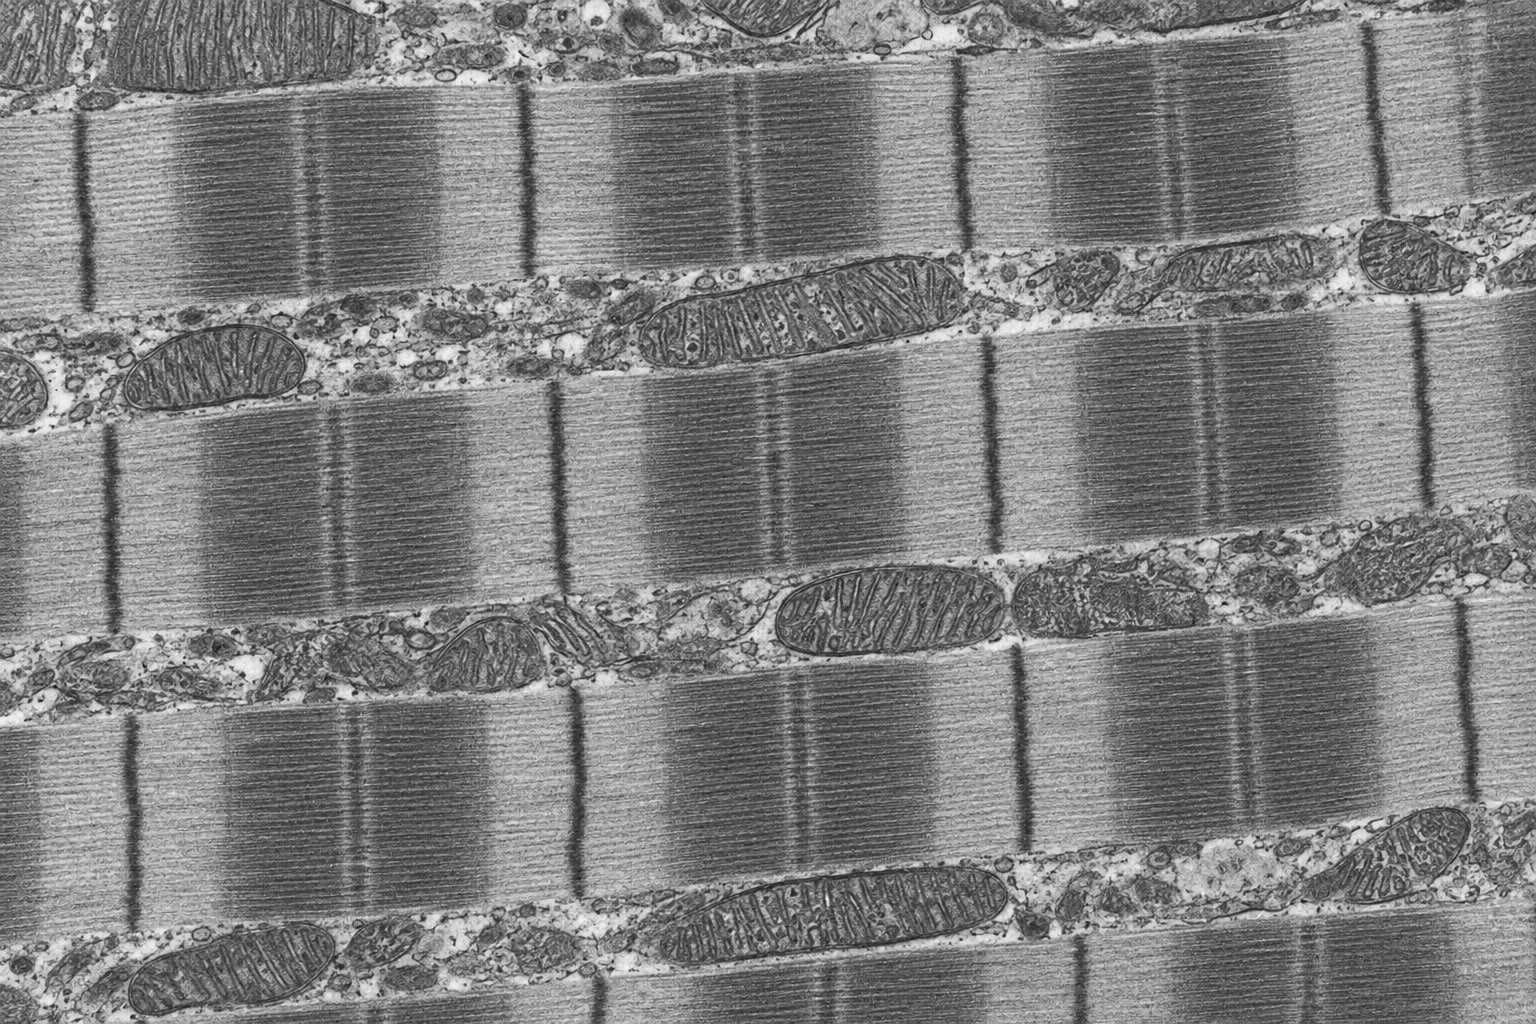
\includegraphics[width=0.6\linewidth]{images/book4/ai/b4-21-sarcomere-tem.jpg}

{\small इलेक्ट्रॉन सूक्ष्मदर्शी के नीचे पेशी-तंतुक: मोटे तंतुओं की A
पट्टियाँ, Z रेखाओं से दो भागों में बँटी पतले तंतुओं की I पट्टियाँ,
और उन तंतुकों के बीच के माइटोकॉन्ड्रिया जो उस सरकने का दाम चुकाते हैं।}
\end{omfigure}

\section{वह मोटर}

\begin{proposition}[अनुप्रस्थ-सेतु चक्र]\label{prop:b2:muscle-movement:crossbridge}
\index{अनुप्रस्थ-सेतु चक्र}\index{मायोसिन}\index{ATP!संकुचन में}
हर मोटे तंतु पर कोई तीन सौ \emph{मायोसिन
शीर्ष} उगे हैं, और हर शीर्ष कोई मोटर है जो चार चरणों के किसी चक्र में
ऐक्टिन के साथ चलता है। (1) ATP बँधी होने पर वह शीर्ष ऐक्टिन से अलग है;
वह उस ATP का ADP तथा फ़ॉस्फ़ेट में जल-अपघटन करता है और स्वयं को किसी
तनी, उच्च-ऊर्जा आकृति में तान लेता है। (2) वह तना शीर्ष किसी ऐक्टिन
उपइकाई से बँधता है, और कोई \emph{अनुप्रस्थ सेतु} बनाता है। (3) फ़ॉस्फ़ेट छूटता है
और वह शीर्ष अपनी ढीली आकृति में चटक जाता है, और उस पतले तंतु को
\omterm{def:b2:cell-differentiation:fibre}{सार्कोमियर} के केंद्र की ओर कोई \qty{10}{nm} खींचता है --- यानी
\emph{शक्ति-आघात}; और ADP निकल जाती है। (4) कोई नई ATP बँधती है और वह शीर्ष
ऐक्टिन को छोड़ देता है; ATP के बिना वह छोड़ नहीं सकता, और वही मृत्यु का
कठोरत्व है। वह चक्र लगभग सेकंड के बीसवें भाग भर लेता है; कोई शीर्ष
उसका अधिकांश अलग रहकर बिताता है, ताकि किसी भी क्षण शीर्षों का केवल कोई अंश
खींचे, और गति से सरकता कोई तंतु कभी छूटे नहीं।
बल जुड़े हुए शीर्षों की खिंचाइयों का योग है; छोटा होना
उनके क़दमों का जोड़ है, अधिक से अधिक प्रति \omterm{def:b2:cell-differentiation:fibre}{सार्कोमियर} प्रति चक्र आधा माइक्रोमीटर;
और वह ऊर्जा प्रति शीर्ष प्रति क़दम एक ATP है, यानी लगभग
\qty{50}{kJ/mol} --- प्रति क़दम \qty{8e-20}{J}, जिसका वह शीर्ष
आधे तक काम में बदल देता है।
\end{proposition}

\begin{omfigure}
\begin{tikzpicture}[every node/.style={font=\scriptsize}, >=stealth]
  \foreach \x/\lab/\ang/\att in {0/{1. ATP बँधी:\\अलग; ATP का\\जल-अपघटन, शीर्ष तना}/60/0, 3.6/{2. तना शीर्ष\\ऐक्टिन से बँधता:\\अनुप्रस्थ सेतु}/60/1, 7.2/{3. फ़ॉस्फ़ेट छूटा:\\शक्ति-आघात,\\तंतु \qty{10}{nm} खिंचा}/20/1, 10.8/{4. ADP निकली, नई\\ATP बँधी: शीर्ष\\छोड़ देता है}/20/0} {
    \begin{scope}[xshift=\x cm]
      \draw[thick, omDef] (0,2.2) -- (2.8,2.2); \foreach \i in {0.2,0.6,...,2.6} \fill[omDef!50] (\i,2.2) circle (0.14);
      \draw[line width=3pt, omExo!80!black] (0,0.4) -- (2.8,0.4);
      \draw[very thick, omThm] (1.4,0.4) -- (1.4,1.0);
      \ifnum\att=1 \draw[very thick, omThm] (1.4,1.0) -- ++(\ang:1.15); \fill[omThm] (1.4,1.0) ++(\ang:1.15) circle (0.16); \else \draw[very thick, omThm] (1.4,1.0) -- ++(\ang:1.0); \fill[omThm] (1.4,1.0) ++(\ang:1.0) circle (0.16); \fi
      \node[below, align=center] at (1.4,0.15) {\lab};
    \end{scope}
  }
  \draw[->, thick, omDef] (7.9,2.55) -- (8.9,2.55); \node[omDef, above] at (8.4,2.6) {पतला तंतु चलता है};
\end{tikzpicture}

{\small \omterm{prop:b2:muscle-movement:crossbridge}{अनुप्रस्थ-सेतु चक्र}। कोई तना मायोसिन शीर्ष (लाल)
ऐक्टिन (नीला) से बँधता है, फ़ॉस्फ़ेट छोड़ता है और उस पतले तंतु को अपने
शक्ति-आघात भर खींचता है, फिर कोई ताज़ी ATP बाँधता है और छोड़ देता है।}
\end{omfigure}

\begin{theorem}[किसी पेशी का बल, गति और शक्ति]\label{thm:b2:muscle-movement:hill}
\index{बल--वेग वक्र}\index{पेशी-शक्ति}
किसी पेशी का बल गिरता है ज्यों-ज्यों वह तेज़ छोटी हो, क्योंकि वे तंतु
जितनी तेज़ सरकें, किसी भी क्षण उतने ही कम शीर्ष जुड़े होते हैं
और उतने ही अधिक अपने आघात से आगे घसीटे जाते हैं इससे पहले कि वे छोड़
सकें। हिल का संबंध उसका वर्णन करता है:
\[
(F + a)(v + b) = (F_0 + a)\,b,
\]
जिसमें $F_0$ समआयामी बल है ($v = 0$ पर), $v_{\max} =
F_0 b/a$ बिना भार की गति, और $a$, $b$ स्थिरांक ($a \approx
F_0/4$)। शक्ति $Fv$ दोनों सिरों पर शून्य है और लगभग
$v_{\max}$ के एक तिहाई तथा $F_0$ के एक तिहाई पर सबसे बड़ी --- और इसीलिए कोई साइकिल-सवार
गियर बदलता है और किसी धावक की डग की कोई पसंदीदा दर होती है। कोई मानव
पेशी अनुप्रस्थ काट के प्रति वर्ग सेंटीमीटर लगभग \qty{30}{N} बल
विकसित करती है, प्रति सेकंड दस लंबाइयों तक छोटी होती है, और अपने सर्वोत्तम पर
प्रति किलोग्राम कोई \qty{100}{W} देती है।
\end{theorem}
\begin{proof}
हिल का वक्र आनुभविक है (1938), जो किसी अलग की हुई मेंढक-पेशी पर
उठाए गए भार के सापेक्ष छोटे होने की गति के रूप में मापा गया; और वह अतिपरवलय
इसलिए बैठता है कि जुड़े शीर्षों का अंश सरकने की गति के साथ गिरता है
और हर जुड़े शीर्ष का बल गिरता है ज्यों-ज्यों वह अपने आघात भर
ढोया जाए। शक्ति: $F = (F_0 + a)b/(v + b) - a$ के साथ, $Fv$
$v = 0$ पर और $v_{\max}$ पर शून्य है; अवकलन करने से वह अधिकतम
$v = b(\sqrt{(F_0 + a)/a} - 1)$ पर मिलता है, जो $a = F_0/4$ के लिए $v =
1.24\,b = 0.31\,v_{\max}$ है, जहाँ $F = 0.31\,F_0$।
\end{proof}

\begin{omfigure}
\begin{tikzpicture}
\begin{axis}[
  width=0.7\linewidth, height=5.4cm,
  axis x line=bottom, axis y line=left,
  xmin=0, xmax=1.05, ymin=0, ymax=1.1,
  xlabel={छोटे होने की गति $v/v_{\max}$}, ylabel={बल $F/F_0$, शक्ति (सापेक्ष)},
  xlabel style={font=\small, at={(axis description cs:0.5,-0.13)}, anchor=north},
  ylabel style={font=\small},
  tick label style={font=\small}, xtick={0,0.31,1}, xticklabels={0,0.31,1}, ytick={0,0.31,1}, yticklabels={0,0.31,1},
  legend style={font=\scriptsize, at={(0.97,0.95)}, anchor=north east, draw=none},
  clip=false,
]
\addplot[very thick, omDef, domain=0:1, samples=100] {(1.25*0.25)/(x+0.25) - 0.25};
\addlegendentry{बल}
\addplot[very thick, omThm, domain=0:1, samples=100] {10.4*x*((1.25*0.25)/(x+0.25) - 0.25)};
\addlegendentry{शक्ति (पैमाना बदला)}
\draw[dashed, gray] (axis cs:0.31,0) -- (axis cs:0.31,1.0);
\end{axis}
\end{tikzpicture}

{\small हिल का \omterm{thm:b2:muscle-movement:hill}{बल--वेग वक्र} ($a = F_0/4$) और जो शक्ति वह
सुझाता है: बल गिरता है ज्यों-ज्यों वह पेशी तेज़ छोटी हो, और शक्ति
अधिकतम गति के लगभग एक तिहाई तथा उस समआयामी बल के एक तिहाई पर शिखर पाती है।}
\end{omfigure}

\section{वह स्विच: कैल्सियम}

\begin{proposition}[उत्तेजन--संकुचन युग्मन]\label{prop:b2:muscle-movement:coupling}
\index{उत्तेजन--संकुचन युग्मन}\index{ट्रोपोनिन}\index{ट्रोपोमायोसिन}\index{पेशीद्रव्यी जालिका}
विश्राम में वे मायोसिन शीर्ष ऐक्टिन तक पहुँच नहीं सकते: पतले तंतु पर
बंधन-स्थल \emph{ट्रोपोमायोसिन} से ढके हैं, यानी कोई ऐसी छड़
जो ऐक्टिन कुंडली की खाँच में पड़ी है और जिसे \emph{ट्रोपोनिन} वहाँ थामे है।
वह स्विच कैल्सियम है। उस तंतु की झिल्ली पर कोई \omterm{prop:b2:neurons-synapses:ap}{क्रिया विभव}
T नलिकाओं से नीचे भीतर दौड़ता है और, उन जोड़ों पर
जहाँ कोई \omterm{def:b2:cell-differentiation:fibre}{T नलिका} \omterm{def:b2:cell-differentiation:fibre}{पेशीद्रव्यी जालिका} से मिलती है, उस
जालिका की कैल्सियम-मोचन वाहिकाएँ खोल देता है; कैल्सियम पेशी-तंतुकों में बाढ़ की तरह आती है,
मिलीसेकंड भर में \qty{0.1}{} से \qty{10}{\micro mol/L} तक चढ़ती है,
ट्रोपोनिन से बँधती है, और ट्रोपोनिन ट्रोपोमायोसिन को उन बंधन-स्थलों से
हटा देता है: वे शीर्ष जुड़ते हैं, और जब तक वह कैल्सियम बनी रहे तब तक वह तंतु सिकुड़ता है।
उस जालिका के पंप, ATP जलाकर, उस कैल्सियम को
दसियों मिलीसेकंडों के भीतर वापस ले लेते हैं; ट्रोपोमायोसिन उन
स्थलों को फिर ढक देता है और वह तंतु ढीला हो जाता है। इसलिए शिथिलन
संकुचन जितना ही सक्रिय है, और ATP से वंचित कोई पेशी न अपने
शीर्ष छोड़ सकती है न अपनी कैल्सियम पंप कर सकती है --- यानी मरण-कठोरता। \omterm{def:b2:heart:anatomy}{हृदय} में वही
स्विच काम में लिया जाता है, पर उस मोचन को छेड़ने के लिए कैल्सियम बाहर से झिल्ली की
अपनी वाहिकाओं से घुसती है, और इसीलिए
\omterm{def:b2:heart:anatomy}{हृदय}, न कि कंकाल पेशी, \omterm{def:b2:blood-circulation:blood}{रक्त} की कैल्सियम के प्रति
संवेदी है।
\end{proposition}

\begin{omfigure}
\begin{tikzpicture}[every node/.style={font=\scriptsize}, >=stealth]
  \node[draw, rounded corners, fill=omDef!15, align=center] (nerve) at (0,0) {प्रेरक तंत्रिका\\आवेग};
  \node[draw, rounded corners, fill=omDef!15, align=center] (nmj) at (3.0,0) {तंत्रिका-पेशी\\संधि:\\ऐसिटिलकोलीन};
  \node[draw, rounded corners, fill=omDef!15, align=center] (ap) at (6.2,0) {पेशी का क्रिया\\विभव, T नलिकाओं\\से नीचे};
  \node[draw, rounded corners, fill=omThm!15, align=center] (ca) at (9.4,0) {पेशीद्रव्यी जालिका से\\Ca$^{2+}$ छूटी};
  \node[draw, rounded corners, fill=omProp!20, align=center] (tn) at (12.6,0) {ट्रोपोनिन Ca$^{2+}$ बाँधता है,\\ट्रोपोमायोसिन हटता है,\\शीर्ष जुड़ते हैं};
  \node[draw, rounded corners, fill=omExo!25, align=center] (off) at (9.4,-2.2) {पंप Ca$^{2+}$ लौटाते हैं (ATP);\\ट्रोपोमायोसिन ऐक्टिन फिर ढकता है:\\शिथिलन};
  \draw[->, thick] (nerve) -- (nmj); \draw[->, thick] (nmj) -- (ap); \draw[->, thick] (ap) -- (ca); \draw[->, thick] (ca) -- (tn);
  \draw[->, thick] (ca) -- (off);
  \node[below, gray] at (1.5,-0.7) {\qty{0.6}{ms}}; \node[below, gray] at (4.6,-0.7) {\qty{1}{ms}}; \node[below, gray] at (7.8,-0.7) {\qty{1}{ms}};
\end{tikzpicture}

{\small तंत्रिका-आवेग से बल तक: वह संधि, उस तंतु का अपना
\omterm{prop:b2:neurons-synapses:ap}{क्रिया विभव}, कैल्सियम का छूटना, और ऐक्टिन-स्थलों का उघड़ना
--- फिर वे पंप जो उसे ख़त्म करते हैं।}
\end{omfigure}

\section{आदेश और श्रेणीबद्धता}

\begin{definition}[प्रेरक इकाई]\label{def:b2:muscle-movement:motorunit}
\index{प्रेरक इकाई}\index{स्फुरण}\index{समाकुंचन}\index{भरती}
मेरुरज्जु में कोई \emph{प्रेरक \omterm{def:b2:neurons-synapses:neuron}{न्यूरॉन}} अपना \omterm{def:b2:neurons-synapses:neuron}{तंत्रिकाक्ष} किसी
पेशी तक भेजता है और शाखित होकर मुट्ठी भर से हज़ार तक
तंतुओं को तंत्रिकित करता है, जो उस पेशी भर बिखरे हैं; और वह \omterm{def:b2:neurons-synapses:neuron}{न्यूरॉन} तथा उसके तंतु
कोई \emph{प्रेरक इकाई} हैं, यानी बल की वह सबसे छोटी मात्रा जिसका तंत्रिका
तंत्र आदेश दे सकता है। उस \omterm{def:b2:neurons-synapses:neuron}{न्यूरॉन} में हर आवेग उस इकाई के हर तंतु को
एक बार दगाता है और कोई \emph{स्फुरण} देता है: यानी ऐसा बल जो
कोई \qty{30}{ms} में चढ़ता है और \qty{100}{ms} में क्षीण होता है, क्योंकि वह
कैल्सियम-स्पंद छोटा है। जल्दी-जल्दी आते आवेग स्फुरणों को
जोड़ देते हैं, क्योंकि अगले के आने तक एक की कैल्सियम पंप नहीं की जा चुकी होती;
और प्रति सेकंड कोई 30 से 50 आवेगों पर वह बल किसी चिकने \emph{समाकुंचन}
में जुड़ जाता है, यानी उस स्फुरण से तीन से पाँच गुना। वह
तंत्रिका तंत्र किसी पेशी का बल दो तरह से श्रेणीबद्ध करता है: उस \emph{दर}
से जिस पर हर इकाई दगे, और उन इकाइयों की \emph{संख्या} से जो वह
भरती करे --- पहले छोटी, धीमी, थकान-रोधी इकाइयाँ
(यानी \emph{आकार-सिद्धांत}), और बड़ी तेज़ इकाइयाँ अंत में, केवल
सबसे बड़े प्रयासों के लिए। इसलिए साधारण काम में कोई पेशी कभी पूरी
चालू नहीं होती: उसकी इकाइयों का कोई अंश दगता है, बारी-बारी, और बाक़ी विश्राम करती हैं।
\end{definition}

\begin{omfigure}
\begin{tikzpicture}
\begin{axis}[
  width=0.82\linewidth, height=5.4cm,
  axis x line=bottom, axis y line=left,
  xmin=0, xmax=1.0, ymin=0, ymax=4.2,
  xlabel={समय (s)}, ylabel={बल (स्फुरण $=$ 1)},
  xlabel style={font=\small, at={(axis description cs:0.5,-0.13)}, anchor=north},
  ylabel style={font=\small},
  tick label style={font=\small}, xtick={0,0.2,0.4,0.6,0.8,1}, ytick={0,1,2,3,4},
  clip=false,
]
% single twitch
\addplot[very thick, omDef, domain=0:0.2, samples=60] {(x<0.02)*0 + (x>=0.02)*4.5*(x-0.02)*exp(-(x-0.02)/0.03)*4.1};
% summation at 10 Hz
\addplot[very thick, omProp, domain=0.25:0.62, samples=200] {(x>=0.25)*4.5*4.1*(x-0.25)*exp(-(x-0.25)/0.03) + (x>=0.33)*4.5*4.1*(x-0.33)*exp(-(x-0.33)/0.03) + (x>=0.41)*4.5*4.1*(x-0.41)*exp(-(x-0.41)/0.03) + (x>=0.49)*4.5*4.1*(x-0.49)*exp(-(x-0.49)/0.03)};
% tetanus at 50 Hz
\addplot[very thick, omThm, domain=0.66:0.98, samples=100] {3.8*(1-exp(-(x-0.66)/0.06))};
\node[font=\scriptsize, anchor=west] at (axis cs:0.09,0.7) {एक आवेग: स्फुरण};
\node[font=\scriptsize, anchor=south] at (axis cs:0.44,2.2) {\qty{12}{Hz}: संकलन};
\node[font=\scriptsize, anchor=south] at (axis cs:0.82,3.85) {\qty{50}{Hz}: जुड़ा समाकुंचन};
\end{axis}
\end{tikzpicture}

{\small दर से बल श्रेणीबद्ध करना। कोई एक आवेग कोई \omterm{def:b2:muscle-movement:motorunit}{स्फुरण} देता है;
प्रति सेकंड दर्जन भर आवेग जुड़कर कोई लहरदार बल देते हैं; और प्रति सेकंड पचास पर
वह बल किसी ऐसे \omterm{def:b2:muscle-movement:motorunit}{समाकुंचन} में जुड़ जाता है जो उस \omterm{def:b2:muscle-movement:motorunit}{स्फुरण} से कई गुना है।}
\end{omfigure}

\begin{proposition}[प्रतिवर्त और मेरुरज्जु]\label{prop:b2:muscle-movement:reflex}
\index{प्रतिवर्त चाप}\index{पेशी-तर्कु}\index{तनाव-प्रतिवर्त}\index{पारस्परिक संदमन}
वह प्रेरक \omterm{def:b2:neurons-synapses:neuron}{न्यूरॉन} \emph{अंतिम साझा पथ} है: हर आदेश,
वल्कुट से हो या किसी प्रतिवर्त से, उसी पर अंत होता है। सबसे सरल परिपथ
\cref{ch:b2:neurons-synapses} का \emph{तनाव-प्रतिवर्त} है:
उस पेशी के भीतर विशेष तंतुओं के चारों ओर लिपटे संवेदी सिरे, यानी वे
\emph{पेशी-तर्कु}, तब दगते हैं जब वह पेशी खींची जाए, और एक ही \omterm{def:b2:neurons-synapses:synapse}{तंत्रिका-संधि} से होकर
उसी पेशी के प्रेरक \omterm{def:b2:neurons-synapses:neuron}{न्यूरॉनों} को उत्तेजित करते हैं, तथा किसी अंतरन्यूरॉन से होकर
प्रतिपक्षी के \omterm{def:b2:neurons-synapses:neuron}{न्यूरॉनों} को संदमित करते हैं
(यानी \emph{\omterm{prop:b2:muscle-movement:reflex}{पारस्परिक संदमन}}), ताकि वह पेशी उस तनाव का
विरोध करे --- यानी मुद्रा का आधार, क्योंकि हर झूल किसी न किसी
पेशी का तनाव है। कोई दूसरा ग्राही, कंडरा-अंग, तब दगता है जब उस
पेशी का बल ऊँचा हो और अपने ही प्रेरक \omterm{def:b2:neurons-synapses:neuron}{न्यूरॉनों} को संदमित करता है: यानी कोई
सुरक्षा-वाल्व। किसी पीड़ादायक उद्दीपन से प्रत्याहरण कई
\omterm{def:b2:neurons-synapses:synapse}{तंत्रिका-संधियों} का कोई प्रतिवर्त है जो उस अंग को मोड़ता है और, दूसरी ओर, दूसरे को
फैला देता है ताकि आप गिरें नहीं। और वह मस्तिष्क
पेशियों को नहीं बल्कि गतियों को आदेश देता है: वल्कुट कोई योजना भेजता है, अनुमस्तिष्क
उसे इसके विरुद्ध सुधारता है कि वे तर्कु क्या बताते हैं, आधारीय गंडिकाएँ उसे
छोड़ती हैं, और मेरुरज्जु के वे परिपथ, जो स्वयं कोई
डग-लय चला सकते हैं, उसे कार्यान्वित करते हैं --- यानी
वर्ष 3 के खंड का विषय।
\end{proposition}

\begin{omfigure}
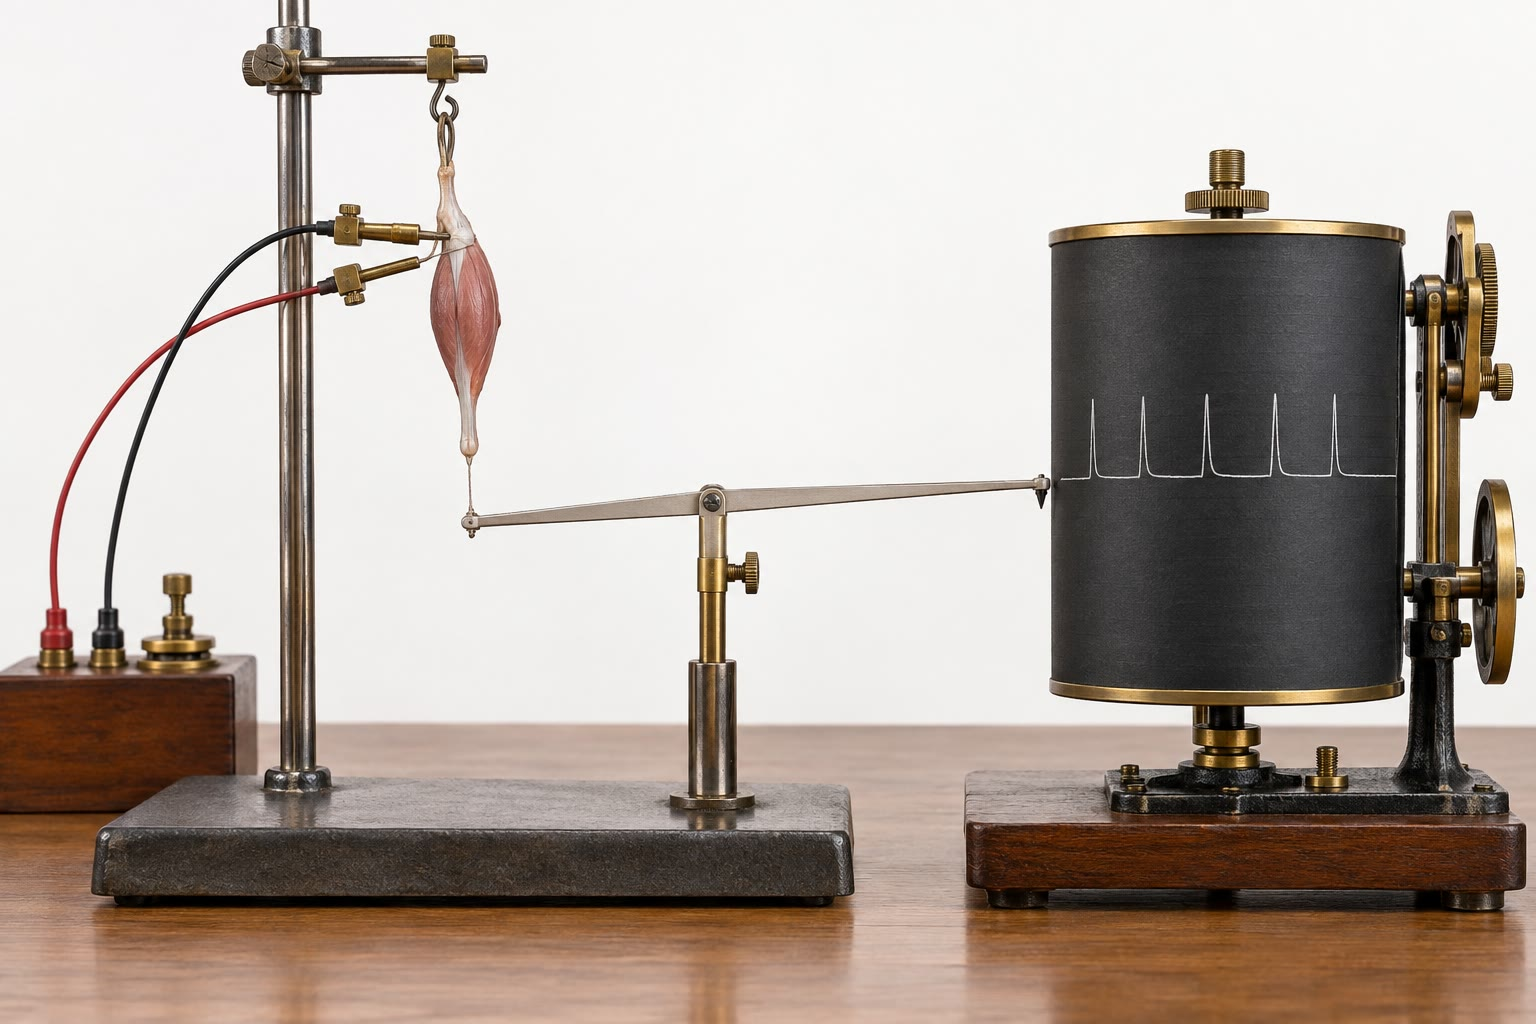
\includegraphics[width=0.44\linewidth]{images/book4/ai/b4-21-frog-muscle-prep.jpg}\hspace{0.04\linewidth}
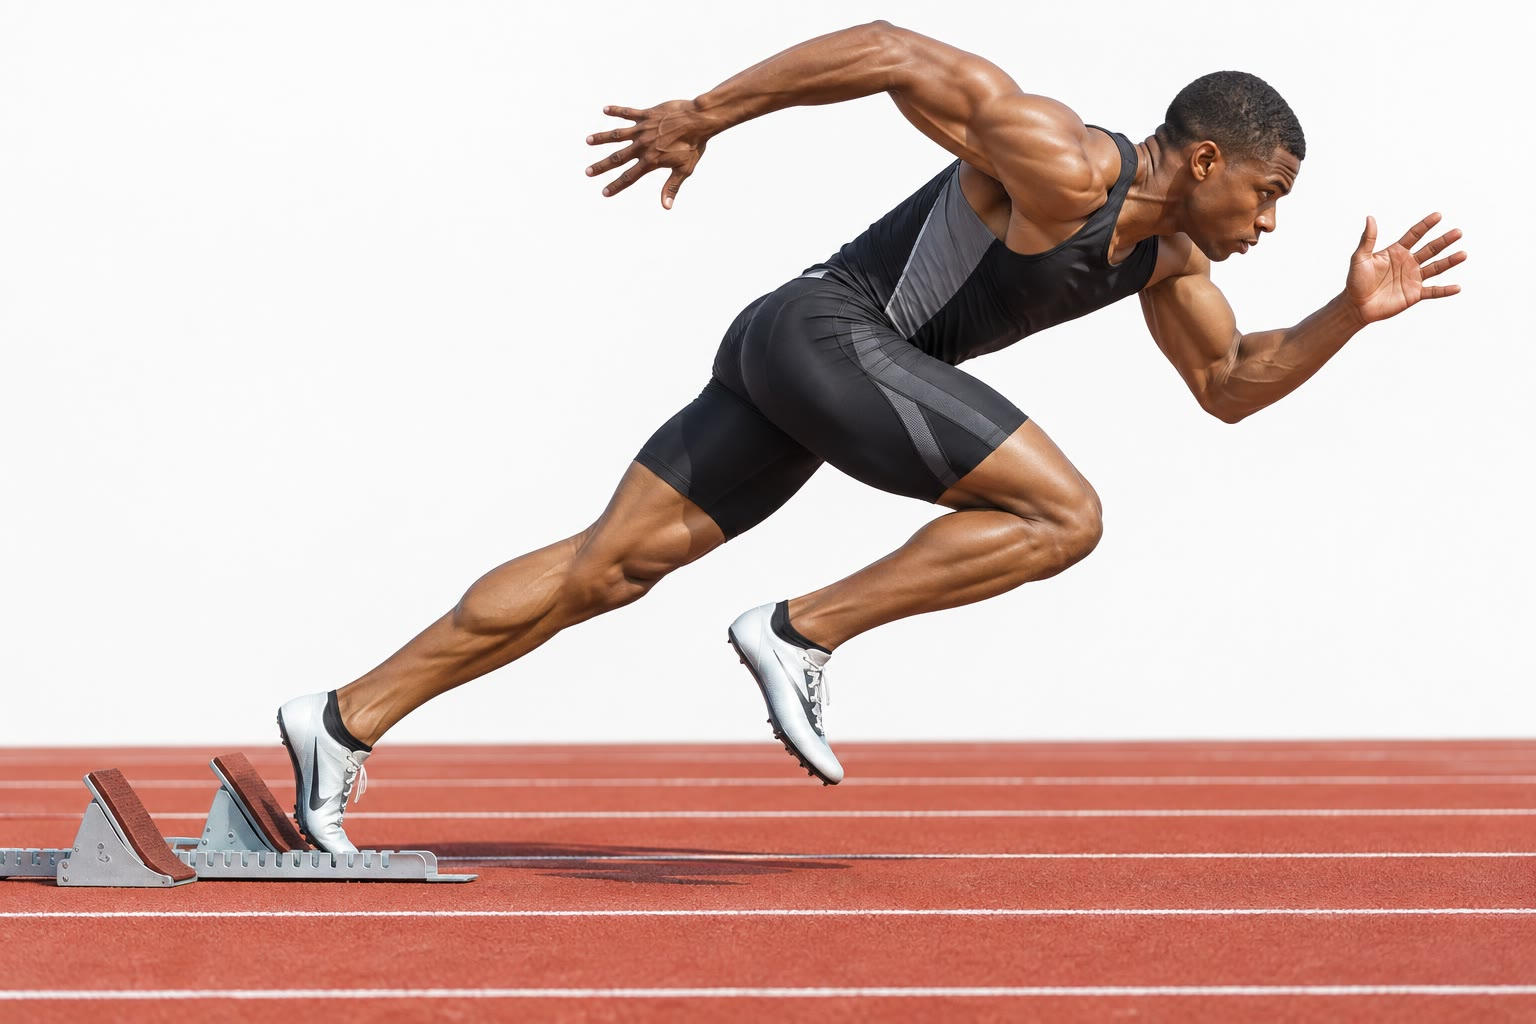
\includegraphics[width=0.44\linewidth]{images/book4/ai/b4-21-sprinter.jpg}

{\small बाएँ: वह चिरपरिचित तैयारी --- कोई मेंढक-पेशी, उसकी
तंत्रिका, उद्दीपक इलेक्ट्रोड और किसी धूमित ढोल पर लिखता कोई उत्तोलक
--- जिस पर \omterm{def:b2:muscle-movement:motorunit}{स्फुरण}, संकलन तथा \omterm{def:b2:muscle-movement:motorunit}{समाकुंचन} पहली बार अभिलिखित हुए।
दाएँ: वही शरीरक्रिया पूरे ज़ोर पर।}
\end{omfigure}

\section{ईंधन और थकान}

\begin{proposition}[उस काम का दाम चुकाना]\label{prop:b2:muscle-movement:energy}
\index{क्रिएटीन फ़ॉस्फ़ेट}\index{पेशी-थकान}\index{ऑक्सीजन-ऋण}
कोई तंतु पूरे ज़ोर के सेकंड-दो सेकंड भर की ATP रखता है। पहला
भंडार \emph{\omterm{prop:b2:muscle-movement:energy}{क्रिएटीन फ़ॉस्फ़ेट}} है, जो ADP का
मिलीसेकंडों के भीतर फिर फ़ॉस्फ़ोरिलन करता है और कोई दस सेकंड चलता है --- यानी धावक का
ईंधन। दूसरा उस तंतु के ग्लाइकोजन का \emph{ग्लाइकोलिसिस} है,
बिना ऑक्सीजन के, जो प्रति ग्लूकोज़ दो ATP तथा लैक्टेट देता है: यानी तेज़,
मिनट-दो मिनट भर को काफ़ी, और अम्ल तथा फ़ॉस्फ़ेट जमा होते ही
स्वयं-सीमित। तीसरा माइटोकॉन्ड्रिया में ग्लूकोज़ तथा
वसीय अम्लों का \emph{ऑक्सीकरणी} उपापचय है, प्रति ग्लूकोज़ तीस ATP, जो केवल
उस ऑक्सीजन से सीमित है जो \omterm{def:b2:blood-circulation:blood}{रक्त} पहुँचाए
(\cref{ch:b2:blood-pressure}): यानी मैराथन। तेज़ ग्लाइकोलिसी तंतु
पहले दोनों पर टिके हैं और मिनट भर में थक जाते हैं; जबकि धीमे ऑक्सीकरणी तंतु,
मायोग्लोबिन से लाल और माइटोकॉन्ड्रिया से ठुँसे, घंटों चलते हैं।
किसी छोटे प्रयास में \emph{थकान} ATP का चुकना नहीं है ---
जो उस पेशी को कठोरत्व में छोड़ देता --- बल्कि
फ़ॉस्फ़ेट तथा प्रोटॉन का जमाव है, जो उन अनुप्रस्थ सेतुओं तथा
कैल्सियम-मोचन को कमज़ोर करते हैं; और किसी लंबे प्रयास में वह ग्लाइकोजन का, और
अंत में, इच्छा का चुकना है। उस प्रयास के बाद वह पेशी अपना
\emph{ऑक्सीजन-ऋण} चुकाती है: वह \omterm{prop:b2:muscle-movement:energy}{क्रिएटीन फ़ॉस्फ़ेट} बहाल करती है, उस
लैक्टेट को वापस बदलती है (यकृत में) और अपने भंडार फिर \omterm{def:b2:muscle-movement:motorunit}{भरती} है, और
निश्चल खड़े रहने के बाद भी मिनटों तक ज़ोर से साँस लेती है।
\end{proposition}

\begin{example}[सौ मीटर]\label{ex:b2:muscle-movement:sprint}
\qty{100}{W/kg} पर \qty{20}{kg} टाँग-पेशी का दस सेकंड का अधिकतम प्रयास
\qty{2}{kW} यांत्रिक शक्ति है और, \qty{25}{\%} दक्षता पर,
ATP-फेर का \qty{8}{kW} --- यानी प्रति सेकंड कोई
\qty{160}{mmol} ATP, या उस दौड़ में \qty{800}{g} ATP।
वह पेशी कोई पचास ग्राम रखती है; \omterm{prop:b2:muscle-movement:energy}{क्रिएटीन फ़ॉस्फ़ेट} पहले
पाँच सेकंड देता है, ग्लाइकोलिसिस बाक़ी, और वह धाविका अपने \omterm{def:b2:blood-circulation:blood}{रक्त} में
\qty{15}{mmol/L} लैक्टेट तथा ऐसा ऋण लेकर पूरी करती है जो वह
अगले पौन घंटे भर चुकाती है। दो घंटे \qty{300}{W} पर कोई मैराथनी
\qty{2}{MJ} काम जलाती है, यानी \qty{8}{MJ} ईंधन --- किलोग्राम भर
ग्लाइकोजन तथा वसा --- और ऑक्सीजन रास्ते भर \qty{4}{L/min} पर
पहुँचती है, और तीसवें किलोमीटर पर वह जिस दीवार से टकराती है वह उसके
ग्लाइकोजन की तली है।
\end{example}

\section{अभ्यास}

\begin{exercise}[$\star$]\label{exo:b2:muscle-movement:1}
\omterm{prop:b2:muscle-movement:sliding}{सरकते-तंतु} क्रियाविधि बताइए और कहिए कि संकुचन पर \omterm{def:b2:cell-differentiation:fibre}{सार्कोमियर} की
कौन-सी पट्टियाँ बदलती हैं और कौन-सी नहीं।
\end{exercise}

\begin{exercise}[$\star$]\label{exo:b2:muscle-movement:2}
\omterm{prop:b2:muscle-movement:crossbridge}{अनुप्रस्थ-सेतु चक्र} के चार चरण और हर एक में ATP की भूमिका
दीजिए। ATP के बिना कोई पेशी कड़ी क्यों हो जाती है?
\end{exercise}

\begin{exercise}[$\star$]\label{exo:b2:muscle-movement:3}
किसी प्रेरक तंत्रिका-आवेग से मायोसिन शीर्षों के जुड़ने तक की घटनाएँ
गिनाइए, और हर एक में लगा काल।
\end{exercise}

\begin{exercise}[$\star$]\label{exo:b2:muscle-movement:4}
\omterm{def:b2:muscle-movement:motorunit}{प्रेरक इकाई}, \omterm{def:b2:muscle-movement:motorunit}{स्फुरण} तथा \omterm{def:b2:muscle-movement:motorunit}{समाकुंचन} की परिभाषा दीजिए, और वे दो रास्ते दीजिए जिनसे
तंत्रिका तंत्र बल श्रेणीबद्ध करता है।
\end{exercise}

\begin{exercise}[$\star\star$]\label{exo:b2:muscle-movement:5}
\qty{2.4}{\micro m} का कोई \omterm{def:b2:cell-differentiation:fibre}{सार्कोमियर} \qty{50}{ms} में छोटा होकर
\qty{2.0}{\micro m} का हो जाता है। मोटे तंतुओं के सापेक्ष पतले तंतुओं की
सरकने की गति निकालिए और, \qty{10}{nm} के किसी क़दम के साथ, वह संख्या
कि हर जुड़ा शीर्ष प्रति सेकंड कितने चक्र करे।
\end{exercise}

\begin{exercise}[$\star\star$]\label{exo:b2:muscle-movement:6}
\qty{10}{cm} के किसी तंतु में श्रेणी में \num{40000} \omterm{def:b2:cell-differentiation:fibre}{सार्कोमियर} हैं और वह
\qty{0.1}{s} में \qty{20}{\%} छोटा होता है। उसके छोटे होने की गति
प्रति सेकंड लंबाइयों में तथा मीटर प्रति सेकंड में, और हर
\omterm{def:b2:cell-differentiation:fibre}{सार्कोमियर} की गति निकालिए।
\end{exercise}

\begin{exercise}[$\star\star$]\label{exo:b2:muscle-movement:7}
हिल के संबंध तथा $a = F_0/4$, $v_{\max} = 10$ लंबाइयाँ प्रति
सेकंड के साथ, प्रति सेकंड 1, 3 तथा 6 लंबाइयों पर बल ($F_0$ के अंश के रूप में)
और हर एक पर शक्ति निकालिए। शक्ति कहाँ सबसे बड़ी है?
\end{exercise}

\begin{exercise}[$\star\star$]\label{exo:b2:muscle-movement:8}
\qty{30}{N/cm^2} पर \qty{80}{cm^2} अनुप्रस्थ काट की कोई जंघास्थि-पेशी:
उसका अधिकतम समआयामी बल निकालिए। वह घुटने के जोड़ से \qty{5}{cm}
दूर किसी ऐसे उत्तोलक पर काम करती है जिसका पैर उस जोड़ से \qty{45}{cm} है:
वह पैर कितना बल लगा सकता है?
\end{exercise}

\begin{exercise}[$\star\star$]\label{exo:b2:muscle-movement:9}
किसी \omterm{def:b2:muscle-movement:motorunit}{स्फुरण} का कैल्सियम-स्पंद \qty{30}{ms} चलता है। समझाइए कि
\qty{10}{Hz} पर आवेग कोई लहरदार बल क्यों देते हैं, \qty{50}{Hz} पर कोई चिकना
\omterm{def:b2:muscle-movement:motorunit}{समाकुंचन}, और वह समाकुंचनी बल उस \omterm{def:b2:muscle-movement:motorunit}{स्फुरण} से बड़ा क्यों है।
\end{exercise}

\begin{exercise}[$\star\star\star$]\label{exo:b2:muscle-movement:10}
किसी धावक की \qty{20}{kg} टाँग-पेशी \qty{25}{\%} दक्षता पर \qty{10}{s} तक
\qty{2}{kW} देती है। काम में ली गई ATP (\qty{50}{kJ/mol}),
पहले \qty{5}{s} को ढकने के लिए ज़रूरी \omterm{prop:b2:muscle-movement:energy}{क्रिएटीन फ़ॉस्फ़ेट}, और
बाक़ी को ढकने के लिए किण्वित ग्लूकोज़ (प्रति ग्लूकोज़ 2 ATP) निकालिए। वह
\qty{40}{L} देह-जल में कौन-सी लैक्टेट सांद्रता डालता है?
\end{exercise}

\begin{exercise}[$\star\star\star$]\label{exo:b2:muscle-movement:11}
इनके संकुचन पर प्रभाव की भविष्यवाणी कीजिए: ऐसी कोई दवा जो उस
जालिका की कैल्सियम-मोचन वाहिका रोके; ऐसी कोई जो उसका पंप रोके; कोई
ऐसा \omterm{def:b2:genome-diversification:mutation}{उत्परिवर्तन} जो ट्रोपोनिन को कैल्सियम के प्रति असंवेदी कर दे; और \omterm{def:b2:blood-circulation:blood}{रक्त} से
कैल्सियम हटाना, कंकाल पेशी के लिए तथा \omterm{def:b2:heart:anatomy}{हृदय} के लिए।
\end{exercise}

\begin{exercise}[$\star\star\star$]\label{exo:b2:muscle-movement:12}
``कोई पेशी ऐसी मशीन है जो रासायनिक ऊर्जा को किसी अच्छे इंजन की दक्षता
और किसी संगणक के नियंत्रण के साथ बल में बदलती है।'' उस दक्षता
(एक चौथाई से आधा) पर विचार कीजिए, कि उसे क्या सीमित करता है, और यह कि
तंत्रिका तंत्र के बल श्रेणीबद्ध करने के दोनों रास्ते वह क्या ख़रीदते हैं
जो कोई अकेला स्विच नहीं ख़रीदता।
\end{exercise}

\section{समस्या: किसी छलाँग की शरीरक्रिया}

\begin{problem}[{सप्तांत समस्या --- खड़े-खड़े की कोई छलाँग सार्कोमियर से
उछाल तक विश्लेषित: वह सरकना, वे अनुप्रस्थ सेतु, वह
कैल्सियम-स्विच, वह बल--वेग सीमा, वे प्रेरक इकाइयाँ तथा वह
ईंधन, और अंत अनुप्रस्थ-सेतु आघातों की संख्या, उस उछाल-गति पर बल, और
वह ATP जो उस छलाँग का दाम है}]
\label{pb:b2:muscle-movement:1}
\qty{70}{kg} का कोई व्यक्ति सीधे ऊपर \qty{40}{cm} छलाँगता है, और
\qty{0.3}{s} के किसी धक्के के दौरान देह के द्रव्यमान-केंद्र को \qty{0.4}{m} चढ़ाता है।
टाँग-प्रसारक (\qty{20}{kg} पेशी) की कुल
अनुप्रस्थ काट \qty{30}{N/cm^2} पर \qty{500}{cm^2} है; उनके तंतु
\qty{12}{cm} लंबे हैं (\num{48000} \omterm{def:b2:cell-differentiation:fibre}{सार्कोमियर}) और उस धक्के के दौरान
\qty{4}{cm} छोटे होते हैं; और वे जोड़ उस पेशी का छोटा होना
पैर पर \num{10} से गुणा और उसका बल उसी गुणक से बाँट देते हैं। $v_{\max} = 8$ लंबाइयाँ प्रति सेकंड, $a = F_0/4$। हर
मोटा तंतु \num{300} मायोसिन शीर्ष ढोता है; पेशी के प्रति वर्ग सेंटीमीटर $6\times
10^{10}$ मोटे तंतु हैं; कोई आघात
\qty{10}{nm} का है और उसका दाम एक ATP (\qty{8e-20}{J}, \qty{50}{kJ/mol});
दक्षता \qty{40}{\%}। वह पेशी \qty{5}{mmol/kg} ATP तथा
\qty{20}{mmol/kg} \omterm{prop:b2:muscle-movement:energy}{क्रिएटीन फ़ॉस्फ़ेट} रखती है। तंतु \qty{60}{\micro
m} चौड़े हैं। प्रेरक इकाइयाँ: प्रति पेशी-समूह \num{800}, हर एक में \num{50} से
\num{2000} तंतु।

\medskip
\noindent\textbf{भाग I --- वह यांत्रिकी।}
\begin{enumerate}
  \item \qty{40}{cm} चढ़ने के लिए ज़रूरी उछाल-गति
        ($v^{2} = 2gh$), और उछाल पर गतिज ऊर्जा निकालिए।
  \item उस धक्के के दौरान टाँगें ज़मीन पर जो माध्य बल लगाती हैं वह
        निकालिए (\qty{0.4}{m} पर काम उस गतिज ऊर्जा
        धन गुरुत्व के विरुद्ध काम के बराबर है), और उस भार से तुलना कीजिए।
  \item उन प्रसारकों का अधिकतम समआयामी बल और, 10 के उत्तोलक-अनुपात के
        साथ, वह अधिकतम पैर-बल निकालिए जो वह
        दे सकता।
  \item उन तंतुओं के छोटे होने की गति प्रति सेकंड लंबाइयों में
        और $v_{\max}$ के किसी अंश के रूप में निकालिए।
  \item हिल के संबंध से, उस गति पर उपलब्ध बल $F_0$ के किसी अंश के रूप में,
        और उससे मिलता पैर-बल निकालिए।
        क्या वह पेशी अकेले वह छलाँग कर सकती है? बाक़ी कहाँ से
        आता है?
  \item उस धक्के के दौरान माध्य यांत्रिक शक्ति और प्रति किलोग्राम
        प्रसारक शक्ति निकालिए।
\end{enumerate}

\medskip
\noindent\textbf{भाग II --- वे अनुप्रस्थ सेतु।}
\begin{enumerate}[resume]
  \item हर \omterm{def:b2:cell-differentiation:fibre}{सार्कोमियर} कितना छोटा होता है, और उसके तंतु उतना सरकाने के लिए
        हर अर्ध-सार्कोमियर पर \qty{10}{nm} के कितने आघात
        करने पड़ते हैं?
  \item हर अर्ध-सार्कोमियर में सरकने की गति और वह
        संख्या निकालिए कि यदि कोई शीर्ष लगातार जुड़ा रहे तो वह प्रति सेकंड कितने
        आघात करता।
  \item उन प्रसारकों में मायोसिन शीर्षों की संख्या निकालिए।
  \item वह काम निकालिए जो वह पेशी स्वयं करती है (उस
        छलाँग की गति पर उसका बल गुणा उसका छोटा होना), \qty{40}{\%} दक्षता पर
        प्रति आघात काम, और ज़रूरी आघातों की संख्या।
  \item प्रश्न 7 से उपलब्ध संख्या के मुक़ाबले वह प्रति शीर्ष कितने आघात
        है? उस भंडार पर टिप्पणी कीजिए।
  \item उस छलाँग में खपी ATP मोलों में तथा ग्रामों में
        (\qty{507}{g/mol}) निकालिए, और उस ATP की ऊर्जा से वह दक्षता जाँचिए।
\end{enumerate}

\medskip
\noindent\textbf{भाग III --- वह स्विच और वह आदेश।}
\begin{enumerate}[resume]
  \item वह धक्का \qty{0.3}{s} लेता है और एक आवेग का कैल्सियम-स्पंद
        \qty{30}{ms}। कौन-सी दगने की दर उन तंतुओं को
        \omterm{def:b2:muscle-movement:motorunit}{समाकुंचन} में रखती है, और हर प्रेरक \omterm{def:b2:neurons-synapses:neuron}{न्यूरॉन} कितने आवेग भेजता है?
  \item \qty{5e-10}{L} के किसी तंतु में मुक्त कैल्सियम \qty{0.1}{} से
        \qty{10}{\micro mol/L} तक चढ़ती है। वह कितने मुक्त कैल्सियम आयन
        हैं, और उन्हें वापस लेने का दाम कितने पंप-चक्र
        (प्रति ATP दो आयन) है?
  \item उन प्रसारकों में तंतुओं की संख्या और प्रति तंतु प्रति आवेग
        अनुप्रस्थ-सेतु ATP निकालिए, और प्रश्न 14 की
        पंप-लागत से तुलना कीजिए। पंप करने की असली लागत उस पेशी की ATP का लगभग
        एक चौथाई है: वह मुक्त कैल्सियम किसे कम आँकती है?
  \item वह तंत्रिका तंत्र इकाइयाँ आकार से \omterm{def:b2:muscle-movement:motorunit}{भरती} करता है। उस छलाँग के लिए,
        कौन-सी इकाइयाँ और किस क्रम में \omterm{def:b2:muscle-movement:motorunit}{भरती} होती हैं? कोई हल्का क़दम उन
        \num{800} में से कौन-सा अंश काम में लेता?
  \item समझाइए कि कम प्रयास पर वह बल बारीकी से क्यों श्रेणीबद्ध हो सकता है और
        अधिकतम के पास केवल मोटे तौर पर।
  \item ऐसी किसी दवा पर कोई व्यक्ति जो \omterm{prop:b2:neurons-synapses:integration}{तंत्रिका-पेशी संधि} को
        आधा रोक दे: उस \omterm{def:b2:muscle-movement:motorunit}{स्फुरण}, उस \omterm{def:b2:muscle-movement:motorunit}{समाकुंचन} तथा उस छलाँग की भविष्यवाणी कीजिए।
\end{enumerate}

\medskip
\noindent\textbf{भाग IV --- वह ईंधन।}
\begin{enumerate}[resume]
  \item उन प्रसारकों में संचित ATP निकालिए और उस
        छलाँग की खपत से तुलना कीजिए।
  \item \omterm{prop:b2:muscle-movement:energy}{क्रिएटीन फ़ॉस्फ़ेट} भंडार और उन छलाँगों की संख्या निकालिए
        जिनका वह दाम चुका सके।
  \item लगातार दस छलाँगें: कौन-सा ईंधन सँभालता है, और क्या
        जमा होता है?
  \item \omterm{def:b2:blood-circulation:blood}{रक्त} उन प्रसारकों तक मिनट भर में \qty{2}{L} ऑक्सीजन
        पहुँचा सकता है (प्रति $\mathrm{O_2}$ 6 ATP)। उस छलाँग की शक्ति को
        कौन-सा ATP-फेर चाहिए, और उसके लिए कौन-सी ऑक्सीजन-आपूर्ति
        लगती? निष्कर्ष निकालिए।
  \item उन छलाँगों के बाद वह व्यक्ति मिनट भर ज़ोर से साँस लेता है।
        काम में ली गई \omterm{prop:b2:muscle-movement:energy}{क्रिएटीन फ़ॉस्फ़ेट} तथा ATP फिर से बनाने के लिए ज़रूरी ऑक्सीजन
        (प्रति $\mathrm{O_2}$ अणु \qty{6}{ATP}) निकालिए और
        \qty{250}{mL/min} की विश्राम-खपत से तुलना कीजिए।
  \item ATP का इतनी दर से फेर होने पर भी किसी छलाँगने वाले की पेशी
        कठोरत्व में क्यों नहीं जाती?
  \item परिणाम बताइए: प्रति अर्ध-सार्कोमियर आघात, उस छलाँग की गति पर
        बल-अंश, और वह ATP जो उस छलाँग का दाम है।
\end{enumerate}
\end{problem}
